\section{Chain Complexes}
\label{sec:Chain Complexes}
\begin{definition}
	A \emph{(non-negative) chain complex} $C$ is a collection of abelian groups $C_n$, $n \in \N$, together with group homomorphisms $\del_n: C_n \to C_{n-1}$, which we call \emph{boundary homomorphisms}, such that $\del_n \circ \del_{n+1} = 0$ for all $n \in \Np$.
\end{definition}

Thus graphically a chain complex $C$ can be depicted by the following diagram:
\begin{center}
\begin{tikzpicture}
	\matrix (m) [matrix of math nodes]{
		\cdots & C_4 & C_3 & C_2  & C_1 & C_0 \\
	};
	\foreach \d/\i/\j in {5/1/2,4/2/3,3/3/4,2/4/5,1/5/6} \path[->] (m-1-\i) edge node[auto] {$ \del_\d $} (m-1-\j);
\end{tikzpicture}
\end{center}

There are many variants to this notion. For example, there are also unbounded chain complexes with an abelian group for each $n \in \Z$ instead of $\N$. In this thesis we will only need chain complexes in the sense of the definition above. Hence we will simply call them chain complexes, instead of non-negative chain complexes. Other variants can be given by taking a collection of $R$-modules instead of abelian groups. Of course not any kind of mathematical object will suffice, because we need to be able to express $\del_n \circ \del_{n+1} = 0$, so we need some kind of \emph{zero object}. We will not need this kind of generality and stick to abelian groups.

In order to organize these chain complexes in a category, we should define what the maps are. The diagram above already gives an idea for this.
\begin{definition}
	Let $C$ and $D$ be chain complexes, with boundary maps $\del^C_n$ and $\del^D_n$ respectively. A \emph{chain map} $f: C \to D$ consists of a family of maps $f_n: C_n \to D_n$, such that they commute with the boundary operators: $f_n \circ \del^C_{n+1} = \del^D_{n+1} \circ f_{n+1}$ for all $n \in \N$, i.e. the following diagram commutes:
	\begin{center}
	\begin{tikzpicture}
		\matrix (m) [matrix of math nodes]{
			\cdots & C_4 & C_3 & C_2  & C_1 & C_0 \\
			\cdots & D_4 & D_3 & D_2  & D_1 & D_0 \\
		};
		\foreach \d/\i/\j in {5/1/2,4/2/3,3/3/4,2/4/5,1/5/6} \path[->] (m-1-\i) edge node[auto] {$ \del^C_\d $} (m-1-\j);
		\foreach \d/\i/\j in {5/1/2,4/2/3,3/3/4,2/4/5,1/5/6} \path[->] (m-2-\i) edge node[auto] {$ \del^D_\d $} (m-2-\j);
		\foreach \d/\i in {4/2,3/3,2/4,1/5,0/6} \path[->] (m-1-\i) edge node[auto] {$ f_\d $} (m-2-\i);
	\end{tikzpicture}
	\end{center}
\end{definition}

Note that if we have two such chain maps $f:C \to D$ and $g:D \to E$, then the level-wise composition will give us a chain map $g \circ f: C \to D$. Also taking the identity function in each degree, gives us a chain map $\id : C \to C$. In fact, this will form a category, we will leave the details (the identity law and associativity) to the reader.

\begin{definition}
	$\Ch{\Ab}$ is the category of chain complexes with chain maps.
\end{definition}

Note that we will often drop the indices of the boundary morphisms, since it is often clear in which degree we are working. The boundary operators give rise to certain subgroups, because all groups are abelian, subgroups are normal subgroups.

\begin{definition}
	Given a chain complex $C$ we define the following subgroups:
	\begin{itemize}
		\item the subgroup of \emph{$n$-cycles}: $Z_n(C) = \ker(\del_n: C_n \to C_{n-1}) \nsubgrp C_n$, and
		\item the subgroup of \emph{$0$-cycles}: $Z_0(C) = C_0$, and
		\item the subgroup of \emph{$n$-boundaries}: $B_n(C) = \im(\del_{n+1}: C_{n+1} \to C_n) \nsubgrp C_n$.
	\end{itemize}
\end{definition}
\begin{lemma}
	Given a chain complex $C$ we have for all $n \in \N$:
	$$ B_n(C) \nsubgrp Z_n(C).$$
\end{lemma}
\begin{proof}
	It follows from $\del_n \circ \del_{n+1} = 0$ that $\im(\del: C_{n+1} \to C_n)$ is a subset of $\ker(\del: C_n \to C_{n-1})$. Those are exactly the abelian groups $B_n(C)$ and $Z_n(C)$, so $ B_n(C) \nsubgrp Z_n(C) $.
\end{proof}
\begin{definition}
	Given a chain complex $C$ we define the \emph{$n$-th homology group} $H_n(C)$ for each $n \in \N$ as:
	$$ H_n(C) = Z_n(C) / B_n(C).$$
\end{definition}
\begin{lemma}
	The $n$-th homology group gives a functor $H_n : \Ch{\Ab} \to \Ab$ for each $n \in \N$.
\end{lemma}
\begin{proof}
	Let $f: C \to D$ be a chain map and $n \in \N$. First note that for $x \in Z_n(C)$ we have $\del^C(x) = 0$, so $\del^D(f_n(x)) = 0$, because the square on the right commutes:

	{\centering
	\begin{tikzpicture}
		\matrix (m) [matrix of math nodes, row sep=2em, column sep=2em]{
			\cdots & C_{n+1} & C_n & C_{n-1} & \cdots \\
			\cdots & D_{n+1} & D_n & D_{n-1} & \cdots \\
		};
		\foreach \i/\j in {1/2,2/3,3/4,4/5} \path[->] (m-1-\i) edge node[auto] {$ \del^C $} (m-1-\j);
		\foreach \i/\j in {1/2,2/3,3/4,4/5} \path[->] (m-2-\i) edge node[auto] {$ \del^D $} (m-2-\j);
		\path[->] (m-1-2) edge node[auto] {$ f_{n+1} $} (m-2-2);
		\path[->] (m-1-3) edge node[auto] {$ f_n $} (m-2-3);
		\path[->] (m-1-4) edge node[auto] {$ f_{n-1} $} (m-2-4);
	\end{tikzpicture}\par}

	So there is an induced group homomorphism $f^Z_n : Z_n(C) \to Z_n(D)$ (for $n=0$ this is trivial). Similarly there is an induced group homomorphism $f^B_n : B_n(C) \to B_n(D)$ by considering the square on the left. Now define the map $H_n(f) : x \mapsto [f_n(x)]$ for $x \in Z_n(C)$, we now know that $f_n(x)$ is also a cycle, because of $f^Z_n$. Furthermore it is well-defined on classes, because of $f^B_n$. So indeed there is an induced group homomorphism $H_n(f) : H_n(C) \to H_n(D)$.

	It remains to check that $H_n$ preserves identities and compositions. By writing out the definition we see $H_n(\id)([x]) = [\id(x)] = [x] = \id[x]$, and:
	$$ H_n(g \circ f)([x]) = [g_n(f_n(x))] = H_n(g)([f_n(x)]) = H_n(g) \circ H_n(f) ([x]). $$
\end{proof}

\subsection{A note on abelian categories}
The category $\Ch{\Ab}$ in fact is an \emph{abelian category}. We will only need a very specific property of this fact later on, and hence we will only prove this single fact. For the precise definition of an abelian category we refer to the book of Rotman about homological algebra \cite[Chapter~5.5]{rotman}. The notion of an abelian category is interesting if one wants to consider chain complexes over other objects than abelian groups, because $\Ch{\cat{C}}$ will be an abelian category whenever $\cat{C}$ is abelian.\footnote{However, this generality might not be so interesting from a categorical standpoint, as there is a fully faithful (exact) functor $F: \cat{C} \to \Ab$ for any (small) abelian category $\cat{C}$, called the \emph{Mitchell embedding} \cite{rotman}. This gives a way to proof categorical statements in $\cat{C}$ by proving the statement in $\Ab$.} The property we want to use later on is the following.
\begin{definition}
	A category $\cat{C}$ is \emph{preadditive} if the set of maps between two objects is an abelian group, such that composition is bilinear. In other words: the $\mathbf{Hom}$-functor has as its codomain $\Ab$:
	$$ \Hom{\cat{C}}{-}{-} : \cat{C}^{op} \times \cat{C} \to \Ab. $$
\end{definition}
To see why functoriality is the same as bilinear composition, recall that the $\mathbf{Hom}$-functor in the first variable uses precomposition on maps, and postcomposition in the second variable. By functoriality this should be a group homomorphism, written out this means: $h \circ (g + f) = h \circ g + h \circ f$ for postcomposition, in other words postcomposition is linear. Similar for precomposition. Together this gives bilinearity of $- \circ -$.

Clearly the category $\Ab$ is preadditive, since we can add group homomorphisms pointwise. Furthermore, postcomposition is linear $h \circ (g + f) (x) = h(g(x)+f(x)) = h(g(x)) + h(f(x)) = (h \circ g + h \circ f) (x)$, and similarly precomposition is linear. Using this we can proof the following.
\begin{lemma}
	The category $\Ch{\Ab}$ is a preadditive category.
\end{lemma}
\begin{proof}
	We can add chain maps level-wise. Given two chain maps $f, g: C \to D$, we define $f+g$ as:
	$$ (f+g)_n = f_n + g_n, $$
	where we use the fact that $\Ab$ is preadditive. Note that $f+g$ is also a chain map, since it commutes with the boundary operator. The bilinearity of composition follows level-wise from the fact that $\Ab$ is preadditive.
\end{proof}

Of course given two preadditive categories $\cat{C}$ and $\cat{D}$, not every functor will preserve this extra structure.
\begin{definition}
	Let $\cat{C}$ and $\cat{D}$ be two preadditive categories. A functor $F: \cat{C} \to \cat{D}$ is said to be \emph{additive} if it preserves addition of maps, i.e.:
	$$ F(f + g) = F(f) + F(g). $$
	In other words the functor $F$ induces a group homomorphism: $F : \Hom{\cat{C}}{A}{B} \to \Hom{\cat{D}}{FA}{FB}$.
\end{definition}

\subsection{The singular chain complex}
In order to see why we are interested in the construction of homology groups, we will look at an example from algebraic topology. We will see that homology gives a nice invariant for spaces. We will form a chain complex from a topological space $X$. In this section we will not be very precise, as it will only act as a motivation. However the intuition might be very useful later on, and so pictures are provided to give meaning to this construction.

\begin{definition}
	The \emph{topological $n$-simplex} $\Delta^n$, $n \in \N$, is the set
	$$ \Delta^n = \{(x_0, x_1, \ldots, x_n) \in \R^{n+1} \I x_i \geq 0 \text{ and } x_0 + \ldots + x_n = 1 \} \subseteq \R^{n+1} $$
	endowed with the subspace topology.
\end{definition}

In particular $\Delta^0$ is simply a point, $\Delta^1$ a line and $\Delta^2$ a solid triangle. There are nice inclusions $\Delta^n \mono \Delta^{n+1}$ which we need. For any $n \in \N$ we define:
\begin{definition}
	For $i \in \{0, \ldots, n+1\}$ the $i$-th face map $\delta^i : \Delta^n \mono \Delta^{n+1}$ is defined as
	$$ \delta^i (x_0, \ldots, x_n) = (x_0, \ldots, x_{i-1}, 0, x_{i}, \ldots, x_n) \text{ for all } x \in \Delta^n.$$
\end{definition}

Given a space $X$, we will be interested in continuous maps $\sigma : \Delta^n \to X$, such a map is called a \emph{singular $n$-simplex}. Note that if we have a $(n+1)$-simplex $\sigma : \Delta^{n+1} \to X$ we can precompose with a face map to get a $n$-simplex $\sigma \circ \delta^i : \Delta^n \to X$. This is illustrated in Figure~\ref{fig:diagram_d} for $n=1$.

\begin{figure}[h!]
	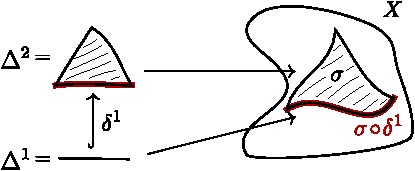
\includegraphics{singular_set}
	\caption{The $2$-simplex $\sigma$ gives rise to a $1$-simplex $\sigma \circ \delta^1$}
	\label{fig:diagram_d}
\end{figure}

From the picture it is clear that the assignment $\sigma \mapsto \sigma \circ \delta^i$ gives one of the faces of the boundary of $\sigma$. If we were able to add these different boundaries ($\sigma \circ \delta^i$, for every $i$), then we could assign to $\sigma$ its complete boundary at once. The free abelian group as defined in the previous section will enable us to do so. However we should note that the topological $n$-simplex is in some way oriented or ordered, which is preserved by the face maps.

\begin{definition}
	For a topological space $X$ we define the \emph{$n$-th singular chain group} $C_n(X)$ by
	$$ C_n(X) = \Z[\Hom{\cat{Top}}{\Delta^n}{X}]. $$
	The \emph{singular boundary operator} $\del : C_{n+1}(X) \to C_n(X)$ is defined on generators as
	$$ \del(\sigma) = \sigma \circ \delta^0 - \sigma \circ \delta^1 + \ldots + (-1)^{n+1} \sigma \circ \delta^{n+1}.$$
\end{definition}

The elements in $C_n(X)$ are called \emph{singular $n$-chains} and are formal sums of \emph{singular $n$-simplices}. Since these groups are free, we can define any group homomorphism by defining it on the generators, the $n$-simplices.

The boundary operator is depicted in Figure~\ref{fig:singular_chaincomplex}. In this picture we see that the boundary of a $1$-simplex is simply its end-point minus the starting-point. We see that the boundary of a $2$-simplex is an alternating sum of three $1$-simplices. The alternating sum ensures that the end-points and starting-points of the resulting $1$-chain will cancel out when applying $\del$ again. So in the degrees 1 and 2 we see that $\del$ is nicely behaved. We will now claim that this construction indeed gives a chain complex, without proof.
\begin{figure}[h!]
	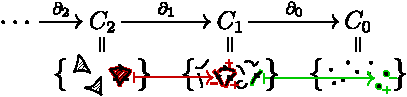
\includegraphics[scale=1.2]{singular_chaincomplex}
	\caption{The boundary of a 2-simplex, and the boundary of a 1-simplex}
	\label{fig:singular_chaincomplex}
\end{figure}

The above construction gives us a functor $C: \Top \to \Ch{\Ab}$ (we will not prove this). Composing with the functor $H_n: \Ch{\Ab} \to \Ab$, we get a functor:
$$ H^\text{sing}_n : \Top \to \Ab, $$
which assigns to a space $X$ its \emph{singular $n$-th homology group} $H^\text{sing}_n(X)$.

With Figure~\ref{fig:singular_homology} we indicate what $H^\text{sing}_1$ measures. In the first space $X$ we see a $1$-cycle $\sigma_1-\sigma_2+\sigma_3$ which is also a boundary, because we can define a map $\tau: \Delta^2 \to X$ such that $\del(\tau) = \sigma_1-\sigma_2+\sigma_3$, hence we conclude that $0 = [\sigma_1-\sigma_2+\sigma_3] \in H^\text{sing}_1(X)$. So this $1$-cycle is not interesting in homology. In the space $X'$ however there is a hole, which prevents a $2$-simplex like $\tau$ te exist, hence $0 \neq [\sigma_1-\sigma_2+\sigma_3] \in H^\text{sing}_1(X')$. This example shows that in some sense this functor is capable of detecting holes in a space.

\begin{figure}[h!]
\begin{subfigure}{.5\textwidth}
  \centering
  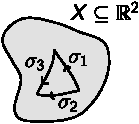
\includegraphics[width=.4\linewidth]{singular_homology1}
  \caption{The $1$-cycle is in fact a boundary.}
\end{subfigure}%
\begin{subfigure}{.5\textwidth}
  \centering
  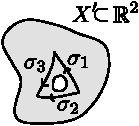
\includegraphics[width=.4\linewidth]{singular_homology2}
  \caption{The hole in $X'$ prevents the $1$-cycle to be a boundary.}
\end{subfigure}
\caption{Two different spaces in which we consider a $1$-chain $\sigma_1-\sigma_2+\sigma_3$, this $1$-chain is in fact a $1$-cycle, because the end-points and starting-points cancel out.}
\label{fig:singular_homology}
\end{figure}

A direct consequence of being a functor is that homeomorphic spaces have isomorphic singular homology groups. There is even a stronger statement which tells us that homotopy equivalent spaces have isomorphic homology groups. So from a homotopy perspective this construction is nice.

In the remainder of this section we will give the homology groups of some basic spaces. It is hard to calculate these results from the definition above, so generally one proves these results by using theorems from algebraic topology or homological algebra, which are beyond the scope of this thesis. So we simply give these results.

\begin{example}
	The homology of the one-point space $\ast$ is given by:
	$$ H^\text{sing}_n(\ast) \iso
	\begin{cases}
		\Z \quad\text{if } n = 0 \\
		0  \quad\text{otherwise}
	\end{cases}. $$
\end{example}
\begin{example}
	Let $S^k$ denote the $k$-sphere (for example $S^1$ is the circle). Its homologyis given by:
	$$ H^\text{sing}_n(S^k) \iso
	\begin{cases}
		\Z \quad\text{if } n = 0 \text { or } n = k \\
		0  \quad\text{otherwise}
	\end{cases}. $$
	For $S^0$ (which consists of only two points) the homology group $H_0(S^0)$ is isomorphic to $\Z \oplus \Z$, and all other homology groups are trivial.
\end{example}

We can use the latter example to prove a fact about $\R^n$ quite easily ($n > 0$). Note that $\R^n - \{0\}$ is homotopic equivalent to $S^{n-1}$, so their homology groups are the same. As a consequence $\R^n - \{0\}$ has the same homology groups as $\R^m - \{0\}$, only if $n=m$. Now if $\R^n$ is homeomorphic to $\R^m$, then also $\R^n - \{0\} \iso \R^m - \{0\}$, so this only happens if $n=m$. This result is called the \emph{invariance of dimension}.
